\documentclass[12pt]{extarticle}
\usepackage{hyperref}
\usepackage{amsmath}
\usepackage{mathtools}
\usepackage{amsfonts}
\usepackage[dvips]{graphicx}
\usepackage{mdframed}
\usepackage[retainorgcmds]{IEEEtrantools}
\usepackage{amssymb}
\usepackage{amsthm}
\usepackage[utf8]{inputenc}
\usepackage[english]{babel}
\usepackage{color}
\usepackage{verbatim}
\usepackage{media9}
\usepackage{xcolor}
\usepackage{titlesec}
\usepackage{makecell}
\usepackage{array}
\usepackage{tabularx}
\usepackage{float}
\usepackage{tikz}
\usepackage{soul}

% Useful definitions for Math environments 
\newtheorem{theorem}{Theorem}[section]
\newtheorem{corollary}{Corollary}[theorem]
\newtheorem{lemma}[theorem]{Lemma}
\theoremstyle{definition}
\newtheorem{definition}{Definition}[section]
\newenvironment{remark}[1][Remark]{\begin{trivlist}
\item[\hskip \labelsep {\bfseries #1}]}{\end{trivlist}}

% For generating subsubsub sections
\setcounter{secnumdepth}{4}
\titleformat{\paragraph}
{\normalfont\normalsize\bfseries}{\theparagraph}{1em}{}
\titlespacing*{\paragraph}
{0pt}{3.25ex plus 1ex minus .2ex}{1.5ex plus .2ex}

% For replacing red link boxes with sturdy colors
\hypersetup{
    colorlinks,
    linkcolor={red!50!black},
    citecolor={blue!50!black},
    urlcolor={blue!80!black}
}
  
% Defining the Art path
\graphicspath{{./images/}}

% Container for tabularx
\floatstyle{plain}
\newfloat{tabcontainer}{thp}{lop}
\floatname{tabcontainer}{Table}

% Container for tikz flow-charts
\floatstyle{plain}
\newfloat{fccontainer}{thp}{lop}
\floatname{fccontainer}{FlowChart}

% For visual representation of Flow-Charts
\usetikzlibrary{shapes.geometric, arrows}
\tikzstyle{startstop} = [rectangle, rounded corners, minimum width=3cm, minimum height=1cm,text centered, draw=black, fill=red!30]
\tikzstyle{process} = [rectangle, minimum width=3cm, minimum height=1cm, text centered, draw=black, fill=orange!30]
\tikzstyle{arrow} = [thick,->,>=stealth]


\begin{document}

\tableofcontents

\section{Definitions}
This section consists of abstractions which will be summoned in the rest of the material.  Please try to be as cooperative as possible with them.

\begin{definition}
  A \emph{Society} is a form? consisting of collective \emph{conciousness} of \emph{entities} or \emph{individuals} along with the mecanisms of sustenance for \emph{human} life form.  
  \end{definition}

\begin{definition}
  In \emph{Capitalist} mode of production in a \emph{Society}, the wealth is immense accumulation of commodities.
\end{definition}

\begin{definition}
  \label{def:commodity}
  A \emph{commodity} is an abstraction represented by an \emph{object} such that it
  \begin{itemize}
  \item is outside \emph{human} context
  \item results in human satisfaction
  \item represents collection of \emph{some}\footnote{The nature of some will be revealed elsewhere within these notes.} properties
  \end{itemize} 
\end{definition}

\begin{remark}
  We note that:
  \begin{itemize}
  \item Commodity has two-fold nature, in the sense that, it is object of utility \ref{def:utility}, at the same time, repository of value \ref{def:values} in certain context (we refer to \ref{sec:elemformval}).
  \end{itemize}
\end{remark}

\begin{definition}
  \label{def:utility}
  A \emph{utility} of a commodity is the resultant of physical properties of that commodity.
\end{definition}

\begin{definition}
 \label{def:thing}
  A \emph{thing} is a physical\footnote{Meaning the context obeying ``Laws of Physics''.} product in its entirety.  Examples are silicon chip, figurine, and energy drink.
\end{definition}
Note: every useful thing has two point of views: \emph{qualitative} and \emph{quantitative}.

\begin{definition}
  \label{def:usevalue}
  The utility of a thing makes the thing a \emph{use value}.  And now the same thing is ``product of labor'' in the context of society.
  \end{definition}

  \begin{lemma}
    Commodity is a use value.
    \end{lemma}
  \begin{proof}
    From definitions \ref{def:thing} and \ref{def:usevalue} it is easy to see that once we use the qualitative(?) viewpoint, commodity is essentially a use value.
  \end{proof}
  \begin{remark}
    We note that use value is now a property of the commodity defined in definition \ref{def:commodity}.  Further more we demand/observe that the use value
    \begin{itemize}
    \item (\textcolor{blue}{Schezophrenia Alert!!!}) is \textbf{completely} independent of the amount of \textcolor{red}{labor}(needs clarification on the definition here) spent into the commodity to appropriate its properties.  Not really sure if Karl is referring to use value or the virtue that utility of commodity manifests itself as use value that is independent of the labor.
    \item  is associated with \emph{definite} quantities for instance couple of transistors, six-pack of monster drink, and dozen of static meshes.
    \item is for gauging the commercial knowledge associated with the commodity.
    \item becomes reality \emph{only} on consumption.
    \item constitute the substance of all wealth (irrespective of the social form of the wealth).
    \item A thing can be a use value to its producer, and product of human labor, without being a commodity.
      \item In order for that product to become commodity, it must have use value for \emph{others}.  Note that this is in concurrence with the definition \ref{def:commodity}.
    \end{itemize}
  \end{remark}

  \begin{definition}
    \label{def:exchval}
    \emph{Exchange value} is a quantitative relation which relates the value of one sort to that of other.\footnote{Here we have defined exchange value in very generic form.  No reference to previous terminologies is supposed to be invoked.}  The relation constantly changes with \emph{time} and \emph{place}.
  \end{definition}

  \begin{remark}
    We note that
    \begin{itemize}
    \item Exchange value \emph{appears} to be something accidental.
    \item Purely \emph{relative}.
    \item One sort can have different exchange values depending on what other sorts it is being compared with.
    \item A \emph{natural} step would be to assume exchange values be transitive.
      \item I suspect that the existence of multiple commodities in the same context gives rise to notion of exchange vlaues.
    \end{itemize}
    \end{remark}

    \begin{lemma}
      \label{lemma:exval}
      Exchange value is intrinsic to the commodities.\footnote{It seems in direct contradiction with the statement ``Nothing can have intrinsik value'' \cite{Barbon:777}.}
    \end{lemma}

    \begin{proof}
      It is quite easy to see that.
      \end{proof}

      \begin{remark}
        We note that
        \begin{itemize}
        \item Exchange values arise in the quantitative viewpoint of commodities.
          \item Exchange values are completely independent from use values.
          \end{itemize}
        \end{remark}

        \begin{definition}
          \emph{Human labor} is an abstract property of commodity which is devoid of any qualitative substance\footnote{Getting rid of use values of the product in this context.} and useful character of any definite kind of labor (like that of mason, porter, and weaver) along with their concerete form, and which is common to all the commodities viewed as \emph{product of labor}.
        \end{definition}

        \begin{remark}
        We note that
        \begin{itemize}
        \item the definition is independent of whatever change of hands the commodity goes through.
        \item the defintion is concerned with the commodity as product of labor by virtue of the commodity's essence and not any qualitative viewpoint.
        \item human labor is \emph{homogeneous} with respect to the commodity.
        \end{itemize}
      \end{remark}

      \begin{definition}
        \label{def:labpow}
        \emph{Labor-power} is a reservior or collective abstraction of human labor, which exists in the organism of every ordinary individual.
      \end{definition}
      \begin{remark}
        We note that:
        \begin{itemize}
        \item This definition seems out of the blue, but since we are not much versed in biology, the words taken as face-value should serve aptly for these notes.
        \item Conversely, organism of every ordinary individual can be viewed as container of the average labor-power\footnote{Within the context of Society.}.
          \item In a society, the organism at certain post for instance air chief marshal etc play a specified \emph{role}, on the other hand, is merely a man/woman (?), a shabby role\footnote{As put forward by Karl.} as a mere human labor.
        \end{itemize}
      \end{remark}
      
      \begin{definition}
        \label{def:values}
        \emph{Values} are mere congelation (semi-solidification) of homogeneous human labor and labor-power expended irrespective of \emph{mode} of its expenditure.
      \end{definition}

      \begin{remark}
        \label{rem:values}
        We note that
        \begin{itemize}
        \item Karl fished out this definition of Values by some ``Social Substance crystal''.  I need to understand what it exactly is.
        \item At this point he kind of stresses that Values are abstracted from use values.  It simply means, Values and use values are to be treated seperately as abstractions.
          \item It is a commodity form, or a property of commodity?
        \end{itemize}
      \end{remark}

      \begin{lemma}
        \label{lemma:valinexval}
        Values of commodities are expressed/manifest themselves in context of exchange values when commodities are exchanged.
      \end{lemma}

      \begin{proof}
        From definition \ref{def:exchval} (of exchange value) we demand that they be transitive.  As the consequence, when commodities (with of course different exchange values) are exchanged, they would still have a common substance, which we can \emph{naturally} identify as Value. 
      \end{proof}

      \begin{remark}
        We make the folowing statements
        \begin{itemize}
        \item The magnitude of value can be measured by the homogeneous human labor spent on the commodity, which, in turn, is measured by its duration.
        \item The duration can be ``denominated'' by weeks, days, and hours.
          \item Finally, we think and ponder on how to find physical representation of true homogeneous human labor.\footnote{Clearly a procrastinating worker completing the work in indefinite amount of time doesn't enhance the value of commodity.  If anything, it diminishes the value.}  
          \end{itemize} 
        \end{remark}

        \begin{definition}
          The total \emph{labor-power} of a society is the \emph{sum total} of the values of \emph{all} the commodities produced by the same society.  This is the homogenoeus mass of uniform human labor-power.
        \end{definition}

        \begin{remark}
          We note that
          \begin{itemize}
          \item Labor-power is \emph{thought to be} composed of innumerable individual \emph{units}\footnote{\textcolor{red}{The detailed analysis on \emph{unit} should be revealed in the later part of these notes.}}.
            \item Futhermore we assume (in the context of commodity production) that these units are indistinguisahble from each other.  Each representative of \emph{some} average colletive property (of society).
            \item Units instrument the gauging of social standards.  That is, what are the regular working timings and so on.
          \end{itemize}
        \end{remark}
        
        Above discussion begs and then demands the right context for homogeneous human labor representation.  One individual may or maynot be enough, but from experience and Karl's arguments, it \emph{seems}, the right context arises with the \emph{collective contribution} of entities existing in a society.

        Let me explain and elaborate Karl's arguments to generate greater mass appeal!  The substance that generates the value (of commodity) is the uniform expenditure of a unit(?) uniform labor-power in form of homogeneous human labor.  Then given the context of commodity production in a society, the value of a commodity is dictated by the expenditure of human labor-power within the time period\footnote{The period is the one that is \emph{socially necessary} given the socially normal conditions of production with the average degree of skill and intensity prevalant at that time.} resulting from the social standards.  Therefore an individual spending less or more time than that socially gauged magnitude is not really representing the homogenous human labor\footnote{Either he is God or highly irrational person!}.

        \paragraph{Case Study: Spinning Jenny}
        The introduction of power looms in England, around 1765 (\href{https://en.wikipedia.org/wiki/James_Hargreaves}{James Hargreaves}), led to the reduced work for churning yarn into cloth.  Thus, the socially gauged magnitude of time for the commodity production, naturally(?) halved (or some fraction).  On the other hand, the handloom weavers, produced the same commodity in same time as before.  That equates to half of the produce, by social standards, given the same time, thus half the human labor (remember it is homogeneous in all possible ways) expended on handloom materials and cosequently, now, the handloom commodity value is halved.

        \begin{remark}
          We note that
          \begin{itemize}
          \item Since social standards now dictate the time, conditions, and so on for commodity production, we have a context for various possible \emph{social dynamics} to appear and chalk out those standards, which in turn drive the society in \emph{some} direction, in very non-direct sense.
            \item It is easy to see that one of the dynamics can be competition which can and will spark in this context, which can be both blessing and curse\footnote{I take no responsibility for describing competition social dynamics here, because my knowledge is quite incomplete and personally I feel it is highly stupid, in the current form, but existing notion.}.
          \end{itemize}
        \end{remark}

        \begin{lemma}
          As values, all commodities are only definite masses of congealed labor time.
        \end{lemma}
        \begin{proof}
          Easy to visualize from above text and discussions.
        \end{proof}

        Unproved lemma
        \begin{lemma}
          \label{lem:comclass}
          \textcolor{red}{In the context of working standards dictated by social standards, each commodity is to be considered as an average sample of its class.}
        \end{lemma}
        \begin{proof}
          To be chalked out elsewhere, or here elsewhen!
        \end{proof}
        \begin{remark}
          \label{rem:comclass}
          We note that
          \begin{itemize}
          \item I don't know what \emph{class} means here.
          \item This lemma deals with social \emph{viewpoint} of the commodity.
            \item In this context, commodities become indistiguisable \emph{if} produced in the \emph{same amount}\footnote{Karl is not serious about the quality of labor time though, here.  It seems that time is outside to his theory and taken to be granted no matter where it comes from.  I'd say that be dictated by the nature of society.} of time.
          \end{itemize}
        \end{remark}

\section{Origins of Definitions and their contexts}
I won't recommend this section for crash course'ers.  Only if you have enough patience and care, you may proceed.
\subsection{Two-fold nature of labor}
The human labor in abstract can be expressed in
\begin{itemize}
\item use value
\item value
\end{itemize}
of a commodity with very different characteristics.  Karl claims that it is due to the fundamental \emph{two-fold} nature of labor itself when studied in the context of commodities.

Consider two commodities, as use values, as following
\begin{itemize}
\item a coat, $\Phi$
\item 10 yards of linen, $\Xi$
\end{itemize}
and let there be a context\footnote{Later we will identify this context by exchange value or value relation.}, in which
\begin{equation}
  \label{eq:exvalphxi}
  \Phi = 2v \text{ and } \Xi = v,
\end{equation}
where, $v$ is some positive number in $\mathbb{R}$ accompanied by some units\footnote{Since we are already familiar with the notion of exchange values (see \ref{def:exchval}), it is not very difficult to imagine use values having same units.}.

\begin{definition}
  \label{def:usefullabor}
  The labor which is responsible for making a thing (\ref{def:thing}), a use value, is called \emph{useful labor}.
\end{definition}

\begin{remark}
  \label{rem:exval}
  We note that:
  \begin{itemize}
  \item Useful labor maifests itself in the utility of the thing (which makes it a use value).
    \item Useful labor is productive activity of definite kind and exercised with a definite aim.
  \item In the above example, $\Phi$ and $\Xi$ are different from each other, qualitatively, in a generalized context.  This implies that the labor responsible for them, correspondingly, should be of different forms i.e tailoring and weaving.
  \item There is no point of exchange between same (indistinguisahble) use values\footnote{Other than checking/recognizing the nature of social standards in different areas and so on.}, seen from qualitative viewpoint.
  \item It is natural to associate a bijection (?) with different use values and different kinds of useful labor.
  \item This demands a calssification of useful labor according to the order, genus, species, and variety to which they belong in the social division of labor.
    \item\label{it:divoflabor}  In community of commodity production, the qualitative difference of useful labor, existing in variety of forms and carried on independently by \emph{individual} producers with accountability, developes into a system primarily supported by a \emph{structure} called division of labor.
  \end{itemize}
\end{remark}


``\emph{\textcolor{blue}{The division of labor is necessary condition for the commodity production.  The commodity production is not necessary condition for divison of labor.}}''\footnote{This makes me realize that division of labor is a structure rather than a mere condition.  See remark \ref{it:divoflabor}.}

For latter, different factors/systems such as biology may be at play\footnote{Think in evolutionary terms and that might lead to something interesting.}.

``\emph{\textcolor{blue}{The relation between physical product (or use value or commodity?) and labor is invariant of the nature of labor, in the sense, that it might be special, by being independent branch of the social division of labor}}.''

This needs more explaination: the relation is not affected by the circumstance in which the physical product is \emph{new}, out of the context of mode of production generated by the division of labor.  In such case, the nature of human race itself imposes some constraints/incentives to generate a relevant context for the ecapsulation of same product production.

``\emph{\textcolor{blue}{That (physical product) which is not a spontaneous produce of Nature, shall owe their existence to some special productive activity, with a definite aim, that appropriates the naturally occuring materials to particular human wants.}}''

Now, as long as labor's useful labor characterstic is manifest, it is a necessary and Nature imposed condition (constraint, independent of all forms of society) for the existence of human race, without which there is no material exchange between human and Nature, and, consequently, no life.

Let me focus on the things, $\Phi$ and $\Xi$, from value (see definition \ref{def:values}) perspective, which is a measure of the homogeneous human labor and gauged or estimated by $v$\footnote{\textcolor{red}{Strictly speaking, the \emph{value} is not equal to $v$}.  It is an abstract notion, not having any dimension}.  In this quantitative context, an exchange value (see \ref{def:exchval}) is natural (given the context of equations \ref{eq:exvalphxi})
\begin{equation}
  \label{eq:exchange}
  \Phi = 2\cdot\Xi = 2v
\end{equation}

It can be easily seen, as value, that they both objectively represent the same homogeneous labor expressed in some form.  We refer the reader to equation \ref{eq:exchangemean} and relevant context for precise meaning.

It is not too difficult to imagine a state of society in which a single man can take on different useful labors (tailoring and weaving for instance here), alternatively.  So now, the two forms of labor are mere modifications of the same homogeneous labor (invoked in the individual) and not a special function of different individuals/persons(?).  \textcolor{red}{I need to find a conceret defition of special activity.}

\emph{In a Capitalist society, the given portion of human labor is in accordance with the variable demand.}

``\emph{\textcolor{blue}{The homogeneous human labor power \ref{def:labpow} must attain a threshold pitch before it can be expended in multiplicity of modes (representing variety of useful labor).}}''

For experimental and educational purposes, let me consider a self-made notion of \emph{work-field}.  We are already familiar with the homogeneous labor in abstract and the notion of labor-power.  Thus it seems natural to define the collection of containers, of labor-power, along with some mechanism (of establishing a relation\footnote{In simple words, it is ``the human labor is expenditure of labor-power''.}) of extracting the human labor, the work-field.
\begin{remark}
  \label{rem:labnat2fold}
  We note that:
  \begin{itemize}
  \item The simple labor power, averaged over the containers in a society, naturally varies in character in different countries and at different times\footnote{I am impressed, Karl!  You are now considering the nature of time in this critique.}.
  \item Skilled labor is simple labor \emph{intensified}, in some useful manner.  One way is
    \begin{equation}
      \text{given quantity of skill } \geq \text{quantity of simple labor}
    \end{equation}
    I will be making it precise in future.
    \item Skilled/concerete labors of different varieties have a common feature: they are all labor power expended and thus inherit the property of generating Value besides appropriating the physical properties of a commodity.
  \end{itemize}
\end{remark}

Now Karl demonstrates a seemingly general scenario (which checks with other video lectures), \emph{that increase in the use value of commodity leads to the decline of its value} (page 33).  It has to do with the two-fold nature of the labor.  I will need to put put this on rigid mathematical formulation.  I wonder if this has some connection to the Spinning-Jenny demonstration.

\subsection{The form of Value and Exchange Value}
From definition \ref{def:values}, it is clear that values have \emph{reality} in \emph{pure} social context.  Furthermore, we witnessed the expression of commodity values in the context of exchange values \ref{lemma:valinexval}, which is reinforcement of the same idea (that they (values) being substance of social context).  This is the first instance of the inclusion of term ``\emph{\textcolor{red}{money form}}'', synonymous to the varied \emph{bodily} forms of the commodity use value,  as the expression of value.  Let us go back to exchange value equation \ref{eq:exchange} and provide a meaning to it
\begin{equation}
  \label{eq:exchangemean}
  \underbrace{\Phi}_{\text{relative form}} = \underbrace{2\cdot\Xi}_{\text{equivalent form}},
\end{equation}
where $\Phi$ and $\Xi$ represent a coat and 10 yards of linen respectively (the relation of use values).  In this context, besides being pure mathematical formulation\footnote{We imply this to be a usual mathematical equation obeying the assumptions of substitution and equivalence (written \href{https://en.wikipedia.org/wiki/Equality_(mathematics)\#Basic_properties}{here}).}, we say that ``\emph{coat expresses its value in linen}'' by the virtue of exchange value.  Thus the value can be easily expressed in both \emph{relative} and \emph{equivalent} forms which are inseparable and mutually exclusive, within the same context.

\begin{remark}
  \label{rem:valexchvalform}
  We note that
  \begin{itemize}
\item the equations like
\begin{equation}
  \label{eq:tuto}
  \Phi = \Phi,
\end{equation}
are expressing only the indistiguishability of use values, which, from pure mathematics, is obvious, but highly useful and fit for the context of social and working standards touched in remarks \ref{rem:exval} (also mentioned in \ref{lem:comclass} from different context or POV).
\item The summoning of value abstraction nessiciates the notion of exchange value because use value by itself is abstracted from value.
\item Mathematics again comes to our rescue in reversing the relation to
  \begin{equation}
    2\cdot\Xi = \Phi,
  \end{equation}
  and restoring the harmony amongst commodities allowing them to switch roles in whatever fashion the context demands.
  \item From the meaning of equation \ref{eq:exchangemean} it is clear that we can't have same form of value expression on both sides.
  \item We declare that value has two anti-podal forms of expression, namely, relative and equivalent.
\end{itemize}
\end{remark}

In what follows, we would like to understand the the manifestation of value (in the context of commodity exchange) in a quantitative way, thus unearthing the role of society in a very explicit way, enough to introduce the mathematical structure and understand the economical dynamics in a rigid fashion.  In our journey, we will encounter the (in)famous money form and try mold it from pure mathematical standing.

\subsubsection{Nature of \emph{relative} form}
First we revisit the definition of exchange value (or value relation) (see \ref{def:exchval}).  A high-schooler, passionate about Physics, can and will tell you that, in order to compare two quantities, we must first devise the relevant units, on which, comparison can be made\footnote{Length can never be compared with speed or energy (except when you are in High-Energy regime, but that is besides the point).}.  Therefore, a relation like \ref{eq:exchangemean} demands the basic units, if we want the same Physics rigor here.

It is clear that this is a game of contexts, meaning, we are bringing two commodities in a single context of exchange values, using or leveraging the use values (a qualitative view-point).  So we will \emph{fix} the physical dimesion\footnote{If you are unaware of dimensional analysis, please consult \href{https://en.wikipedia.org/wiki/Dimensional_analysis}{this}.} of use values to be $[\omega]$\footnote{I am so tempted to use `uv' initials here, but umm $\ldots$.}.  \textcolor{red}{I have reasons to think that this fixing should hold in general, outside the context of exchange value relations.  I leave it on the time for scrutiny}.

Ok, it turns out I was neglecting the use value as representation of sum of physical properties, which, by the virtue, demands seperate dimensions for different commodities, not brought or existing in the same context.  Hence we will denote the physical dimension of use value to be
\begin{equation}
  \label{eq:usevaldim}
  \left[\Omega_{\text{Commodity Name}}\right]
\end{equation}


The naming convention of units, of dimension $\Omega_{\text{Commodity Name}}$, shall be
\begin{equation}
  \label{eq:nameconvunit}
  \text{`definite number'}\text{`initials of physical measure'}\footnote{Could be something like km, s, or kg}
\end{equation}
Thus for the thing `linen', as it stands alone as commodity, we have a sequence\footnote{Refer the definition \href{https://en.wikipedia.org/wiki/Sequence}{here}.} $\mathbb{S}_{\text{linen}}$ of use values, like so
\begin{equation}
  \label{eq:metricsysuseval}
  \mathbb{S}_{\text{linen}} =  \{\ldots,6\text{yd}, 4\text{yd}, \text{yd}, \ldots\},
\end{equation}
where, `yd' stands for yards, with each element having dimension $\Omega_{\text{linen}}$ and the following usual conversion
\begin{equation}
  \label{eq:usevalconv}
  (6\text{yd})_{\text{linen}} = 6\cdot (\text{yd})_{\text{linen}}.
\end{equation}

If the use value is gauged without any physical measure, then we write `np' for non-physical\footnote{Implying real but not having physical quantity like meters, seconds, ampere etc.}.

Now equipped with this arsnel, we look at equation \ref{eq:exchangemean} again, which translates as follows
\begin{align}
  \label{eq:usevalexeq1}
  \Phi &= 2\cdot \Xi,\\
  \label{eq:usevalexeq2}
  \underbrace{(\text{np})_{\text{coat}}^{\omega}}_{\text{relative form}} &= \underbrace{2\cdot (10\text{yd})_{\text{linen}}^{\omega}}_{\text{equivalent form}}.
\end{align}

Here we have explicitly shown the fixing of use value dimension such that the appropriate comparison is legal\footnote{From pure mathematical POV.}.  In Karl's language, this is equivalent of ``coat=linen'' basis.

\begin{remark}
  \label{rem:relform}
  We note that, in the context of the relation above
  \begin{itemize}
  \item Linen is the mode of existence of Value, implying Value is now ``in-action'', as long as dimension of use value is $\omega$.  Linen is the body of Value now.  I'd like to think Value is \emph{instantiated} on the linen (as equivalent form) by the coat (as relative form), or linen is ``possessed'' by coat, in a useful way.   Thus we have successfully captured the abstract notion of value in a physical form\footnote{Form following Laws of Physics, strictly.}.
  \item On the other hand the value of coat acquires an \emph{independent} expression, in this context, as something comparable and, thus, exchangeable with something different\footnote{Different not in physical sense, in which they really are and we are not interested in that here, but, rather, in the sense of substance (the way its ingredients are arranged?  Borrowing from chemistry especially the example of butyric acid ($CH_3CH_2CH_2CO_2H$) and propyl formate ($CH_3CH_2CH_2OCOH$)) and/or different specialized labor.  \textcolor{red}{I am not sure if this is a necessary condition though}.} of equal value.
  \item The value of coat stands forth in its character by the reason of its relation to the other.
  \item It can also be said, the bodily form of coat is a use value.  Seems out of the blue at the moment, but see page 41 paragraph 3.
  \item This relation also brings forth the nature of labor common to both varieties of specialized labor, responsible for physical existence and value creation of both things, a human labor in the abstract.
    \item It is the human labor power expended, the human labor in the abstract, which generates the value (as per the definition \ref{def:values}).
    \item In order to define value as congealed state of human labor, it must have objective existence, \emph{materially} different from the coat and yet something common to all the commodities.  This is somehow related to the fact that in equation \ref{eq:usevalexeq1}, $\Xi$, as equivalent, represents something more in the bodily form\footnote{Same as physical form, just sounds more extravagant!  I will be using the two terminologies interchangeably, in these notes.}, a dressed thing, when compared with as standalone commodity.  I may need to find mathematical basis for the expression of this!
    \item $\Xi$ is a body of value, depository of human labor (weaving, a shape of human labor power, expended)
    \item When two things are brought in context, say $A$ and $B$, A can't fulfil its role unless $B$ ``sees'' some bodily form of the same role in $A$.  I know how it works, just want to understand its relevance here (look what I did!).  Would be useful to understand in the reflexive scenario!  When $A=B$.
      \item In Karl's fancy description, commodities talk and communicate when brought/written in value relation.  Furthermore, they do that with the human languages including Hebrew, German, and hopefully Sanskrit!  It would be dope to associate Linguistics with Economics, in the form of component, though!
  \end{itemize}
\end{remark}

\begin{definition}
  \label{def:relval}
  In the exchange value or value relation equation (such as \ref{eq:exchangemean}), the value appearing in the relative form is the \emph{relative value} (a real number in $\mathbb{R}$\footnote{An element of real \emph{field}, to be pedantic, which can be refered \href{https://en.wikipedia.org/wiki/Field_(mathematics)}{here}}).
\end{definition}

\begin{remark}
  We note that
  \begin{itemize}
  \item It is important to distinguish and, thus, clarify the meaning of relative value.  The value (see \ref{def:values}), of the commodity in relative form (see \ref{eq:usevalexeq2}), is \emph{expressed} in the use value (see \ref{def:usevalue}) of the commodity in the equivalent from (again see \ref{eq:usevalexeq2}), and we say that the ``value has taken the form of \emph{relative value}''\footnote{It is very important to understand theorem \ref{th:relvalandval} before making any prejuidices about it.}.
  \end{itemize}
\end{remark}

Now relative value is something numerical and we denote it by $v_{\text{coat}}^{r}$.  We consider equation \ref{eq:usevalexeq2} again with a scope of ``kinematics''\footnote{In Physics, kinematics is the analysis of evolving system only in terms of predefined degrees of freedom, with relevant time, without the regard for internal/external influences and backreactions.  The analysis done after solving Equations Of Motion, so to speak!}
\begin{equation}
  \label{eq:valreltestvar}
  (\text{np})_{\text{coat}}^{\omega} = 2\cdot F(\ldots)\cdot (10\text{yd})_{\text{linen}}^{\omega},
\end{equation}
where, $F(\ldots)$ is called \emph{form factor} whose arguments\footnote{We note that this same factor can be quite useful in expressing the dependence of exchange value, of a commodity, on time and place, as merrily noted in \ref{def:exchval}.  I would like to even go further by stating that ``\textcolor{blue}{$F(\ldots)$ is supported on pesudo-Riemannian manifold $(\mathcal{M}, g)$''}.  Here $g$ is the solution to Equations of Motion resulting from the Einstein-Hilbert action.} we will try to determine by variational methods, such that, previous arguments hold, in the context of exchange values.


\begin{itemize}
\item First we demand the following explicit dependence
  \begin{equation}
  v_{\text{coat}}^{r} = F(t_{\text{coat}}^l, \ldots) = a\cdot t_{\text{coat}}^l, 
\end{equation}
where $t_{\text{coat}}^l$ is the amount of time, the human labor (expended human labor power) was congealed for the production of coat.
It is easy to check that once $t_{\text{coat}}^l$ doubles, it has direct effect of same factor in the equation \ref{eq:valreltestvar}.

Conclusion:``\emph{\textcolor{blue}{The value of commodity rises $\Rightarrow$ relative value $v^r$ may\footnote{We will be making weak statements for now, because complete form of $v^r$ is unknown, given the factor $a$.} increase.}}''

\item Next, we demand the following explicit dependence of $a$ like so
  \begin{equation}
    \label{eq:adep}
    a = \lambda\cdot\frac{1}{t_{\text{linen}}^l},
  \end{equation}
  resulting in the equation
  \begin{equation}
    \label{eq:relvalform}
     v_{\text{coat}}^{r} = \lambda \cdot \frac{t_{\text{coat}}^l}{t_{\text{linen}}^l}.
   \end{equation}
   
   Conclusion:``\emph{\textcolor{blue}{The value of commodity remains fixed $\Rightarrow$ relative value $v^r$ may decrease.}}''
 \end{itemize}
 I am doing nothing new, just framing Karl's words in pure mathematics.  The new part is leaving the $\lambda$ as is, because, in future, if we find more factors responsible for value change of a commodity (favorite endeavor for mathematics friends), it would be easy enough to incorporate in this encapsulation of form factor!

 \paragraph{Properties of $v_{\text{Commodity Name}}^{r}$}
 This subsubsub-section is partly less scrutnized, because, I need to do more thinking.

 \begin{theorem}
   \label{th:relvalandval}
 Change in $v^{r}$ (given the mathematical form \ref{eq:relvalform}) is neither necessary nor sufficient condition for reflecting change in the value of the commodity.\footnote{The symbol for relative value, of generic commodity, is written by ommiting the sub-text.}
 \end{theorem}

 From Karl's arguments and common sense, we see if the labor time is increasing simultaneously for both the commodites, in exchange relation \ref{eq:valreltestvar}, in \emph{same direction} and with \emph{same proportions}, then one can easily imagine values of both the commodities increasing but the $v_{\text{coat}}^{r}$, defined in \ref{eq:relvalform}, remains fixed.

 \begin{proof}
   Consider the following (mathematical) variation of relative value (given the expression in \ref{eq:relvalform})
   \begin{align}
     \label{eq:variationdemo}
      \delta v_{\text{coat}}^{r} &= \lambda\frac{t_{\text{linen}}^l\delta{t_{\text{coat}}^l} - t_{\text{coat}}^l\delta{t_{\text{linen}}^l}}{\left(t_{\text{linen}}^l\right)^2}
   \end{align}
   Now as per Karl's arguments if the relevant conditions are met (same direction and same proportion)
   \begin{align}
     \delta{t_{\text{coat}}^l} &= \gamma \delta{t_{\text{linen}}^l},\\
     \gamma &= \frac{t_{\text{coat}}^l}{t_{\text{linen}}^l},
   \end{align}
   it is easy to see that $\delta v_{\text{coat}}^{r}$ vanishes in-spite of $ \delta{t_{\text{coat}}^l}, \delta{t_{\text{linen}}^l} \neq 0$, which represent not-trivial, but simple, human labor time changing the values of commodities written in value relation.

   So we have seen that $\delta v^r = 0$ doesn't necessarily imply constant absolute value of the commodity.  Earlier we saw that even $\delta v^r \neq 0$ doesn't always imply changing absolute value of commodity.
 \end{proof}

 Moving on, since we have discovered the conditions of degenracy in $v_{\text{coat}}^r$, the natural question is: how to revive the relative value?
 Solution is simple, yet involves introduction of more complexity!  That is, bringing third commodity, say pants, in the context of exchange values, whose value is constant.  \textcolor{red}{I think that $v^r$ needs better naming, in terms of all commodities involved!}


\subsubsection{Nature of \emph{equivalent} form}
Let me rewrite the exchange value equation \ref{eq:valreltestvar} to paint the picture.
\begin{equation}
  \label{eq:exvalrep}
   (\text{np})_{\text{coat}}^{\omega} = 2\cdot F(\ldots)\cdot (10\text{yd})_{\text{linen}}^{\omega}.
 \end{equation}
 \begin{remark}
   \label{rem:equiform}
   Since we have fixed the dimension of both the use values as $[\omega]$, we note that, in this context of exchange value (of coat?)
   \begin{enumerate}
   \item Coat expresses its ``quality of having a value'' (relative value $v^r$), in the use value of other commodity (equivalent form), by the fact that coat is still\footnote{The appearance of commodity \emph{in} the specific bodily/equivalent form, of all the forms it could have entered the relation.} in the bodily form (completely explainable as per the Laws of Physics, and ultimately, Nature) and nothing more is required from the relation.
   \item The same bodily form (which one relative or equivalent?) is now the value form (an equivalent form), we say, only when some \emph{other} (product of different kind of labor?) commodity enters the value relation in relative form.
   \item The fact that linen has value is clear from the relation which allows the direct exchange with coat.
   \item Linen, as a seperate commodity, has its value based on the labor time\footnote{And whatnot!  I need to think more about it.}.  But when written in equivalent form, value can't acquire any quantitative form (unlike $v^r$ for relative form)\footnote{What Karl seems to be suggesting is that, when the labor time in equivalent commodity is increased, in the context of this relation, it just diminishes the relative value of relative commodity without expressing itself in equivalent form.  It checks out with the variational kinematics of equation \ref{eq:valreltestvar}.}.  The value magic is gone for the equivalent commodity and, on the other hand, it gained the magic of being in physics realm\footnote{I'd like to think of it as collection of some vibrational mode of (bosonic?) strings, from String Theory.}, as a definite quantity.
   \item \textcolor{blue}{One clue, about bringing two commodities in exchange value context, is the deciding criteria of the ratio (or initial value of form factor $F(\ldots)$) which is the magnitude (whatever it means) of absolute value.}.
   \item We can also see the form factor $F(\ldots)$ as the ``equivalent use value embodiement'' of value (expression in form of $v^r$).
   \item \label{mark:usevalVal} The use value (from which the Value was abstracted\footnote{See Values remark \ref{rem:values}.}) becomes the menifestation of its opposite, the Value.  However keep in mind, use value of equivalent form and Value of relative form of different(?) commodities are being identified.
   \item \label{mark:reflexarg} Now Karl states something I highly disagree with, and this sheds light on the tension between unchecked Economics and mathematical form of Economics\footnote{Compilation of the entire scope in mathematical language, inevitably from first principles.  Axiomatic Economics so to speak, but that would be ambitious.}.  ``No commodity can stand in the (relative) relation of equivalent to itself, and thus turn its own bodily shape into the expression of its own value, every commodity is \emph{compelled} to choose some other commodity \ldots''.  I can't convince myself, especially when I perform a literal \emph{Gedankenexperiment} of standing in front of (physical) mirror and see my reflection.  Here I am the relative form and reflection is equivalent form, which is essentially my body, in some sense, being the mode of my-being (the Value) expression.  If you want mathematical foundation of doubt, refer equation \ref{eq:usevalexeq2}, which by mathematics, should hold \emph{reflexive} property (clearly visible in \ref{eq:tuto}).
   \item \label{mark:combod} The body of the commodity existing in the equivalent form expresses itself as the \emph{materialization} of human labor in the abstract at the same time the product of specifically useful labor (tailoring or weaving) which, I think, is the fact, that Value is being represented in the use value of other (remember the form factor).
     \item It is easy to see and, then go further and, state that ``specialized labor is container of the homogeneous human labor'', the concrete labor becomes medium to express the human labor.  We see another instance of role switch, in which, the conceret labor\footnote{Responsible for generating useful properties of the commodity it is associated with.} of a commodity is now dissociated with it (remember we fixed the dimension to be $[\omega]$ and dissolved its earlier nature) and now aquires a new role, being the mode and form of expression of human labor in the abstract, as long as the value relation holds\footnote{For instance, now (given the value relation)  we say that the utility of weaving consists not in making the cloth, but making an object and hence being creator of Value for coat, for which, it is a mere congeleation of inditiguishable, and thus, homogeneous labor in the abstract.}.  We note that the two-fold nature of labor comes in handy to complete the circle or chain of arguments, in this mirroring scenario.
   \end{enumerate}
 \end{remark}

 \paragraph{Need for \emph{other} commodity}
 \label{par:needforother}
 Commodities of Capitalist mode of production are characteristic of the era, geographic location and nature of society.  Therefore, they have to go through the ``measures'', surviving and, resulting from the passage of ages in a harmonious way, such that there is a robust continum generated, leading to the continuation of life\footnote{We noted earlier, one condition for life could be material exchange between human and Nature.}.

 Now consider a commodity, a sugar-loaf for instance, produced in some recent time-period, whose use values are to be gauged.  It is important to consider the only context of life we know of, planet Earth.  Thus the commodity has to be a product of some surviving and florishing\footnote{I will describe the deep meaning of florishing later, here.} society on Earth.

 Now a Physicist will tell you, on planet Earth, if a something (coinciding with our definition of thing \ref{def:thing}) is heavy, it has weight.  For him, weight is a force given by the equation
 \begin{equation}
   \label{eq:weightphysics}
   W = m\cdot g,
 \end{equation}
 where $m$ is the mass (heavyness) and $g$ is acceleration due to gravity on Earth (9.8 m/sec/sec).  The units of the force is Newtons.

 But our friend Karl uses the same word ``weight'' with more context, so it seems.  Because once a commodity is presented, it should have weight given by same equation \ref{eq:weightphysics}, no matter produced this century or Before Common Era and nothing more should be required for Physics analysis.  Karl suggests that there is still something unknown about the weight.  ``We can neither see or touch this weight'' he observes.  Physicists have no issue with this statement, but when Karl brings in pieces of iron in this context, with the thought ``whose weight has been determined beforehand'', then Physicists feel something new has to be formulated in order to capture that something unknown, hidden from Physical analysis for over 400 years.

 ``\emph{\textcolor{orange}{The iron, as iron, is no more the form of manifestation of weight, than is the sugar-loaf. Nevertheless, in order to express the sugar-loaf as so much weight, we put it into a weight-relation with the iron}}''

 I wouldn't care much about it, but if it were not for the phrase ``in order'', which implies consideration of some division (of labor?) in the mode of production, being leveraged to assess the commodity's physical weight.  Even Karl is not explicit enogh to talk about that something more, but instead outsources that part of the context to some well conceieved notion of the weight of the iron pieces\footnote{What ever that means, says the Physicists inside me.}.  This works and reinforces our vision of society with iron pieces playing the role of measures.

 The purpose here is to draw an analogy with the precise physical measurements (you know using the entire physics machinery), but by being honest to the observational Economic phenomenons\footnote{Who knows, just like Mahtematics, Economics might allow the interplay with Physics.}.  Therefore we will allow Karl's context of weight to go through the physics machinery, for him to be able to prove a point.  And in return, we will get clear distinction between Nature, human, and social contexts.

 What follows, Karl names the ``weight-relation'', in which, sugar-loaf (as a physical thing) is to be measured by iron pieces, in terms of weight (as whatever you understood from previous discussion of this section, which is certainly more than \ref{eq:weightphysics}).  So certain quantity of iron officiates, the relation, as a body representing nothing but the weight\footnote{Remember it was assumed to be a measure \emph{earlier}.} or the form of manifestation of weight.  We say\footnote{Based on Karl's statemets\newline ``\emph{\textcolor{blue}{A certain quantity of iron therefore serves as the measure of the weight of the sugar,
and represents, in relation to the sugar-loaf, weight embodied, the form of manifestation of
weight. This part is played by the iron only within this relation, into which the sugar or any other body, whose weight has to be determined, enters with the iron. Were they not both heavy, they
could not enter into this relation, and the one could therefore not serve as the expression of the
weight of the other.}}''} that, now, Physics is completely capturing all the information of the context.  By the way I have no issue with throwing in the iron as the other commodity here.  If anything, it implies and then justifies the self consistency checks, meaning equation \ref{eq:tuto}, and my disagreement with Karl's argument noted earlier.

If you are still maintained, in these notes, we have the moment of truth
``\emph{When we throw both into the scales, we see in reality, that as weight they are
  both the same, and that, therefore, when taken in proper proportions, they have the same weight.}''

The lesson we learn from this exercise, is that (certain quantity of?) iron started off as a measure, switched its role exclusively to the embodiement of weight (still something more than Physics definition) when in \emph{physical relation} with the sugar-loaf.  And just like that, we uplift this notion to Karl's satifaction, and declare that ``in the value relation, the equivalent form is a mode of an expression of Vale, exclusively''.


\paragraph{Distinction between Nature and society}
However, Karl marks a clear (and absolute, if I might add) distinction between the \emph{naturalness} of weight\footnote{And still I note the more context of weight, than gauged by Physics.} in the physical relation and \emph{non-naturalness}, purely social (nature?), of Value (of the commodity in relative form) being expressed in the use value of equivalent form, in value relation.  We note that the notion of equivalent-relative form itself maybe purely mathematical, but the abstractions expressed themselves are categorised into natural and social.

The relative form of the commodity expresses the Value of the commodity as being wholy different from its substance (as noted in the remarks \ref{rem:relform}) and (physical?) properties.  A value relation, by itself, suggests that some social relation (that both are constituents of labor) is underlying in the virtue of the equation (essentially the whole context of bringing commodities together).  On the other hand, the same Value (of the commodity in relative form), is expressed in the materialistic properties (or the bodily form) of the commodity in equivalent form, which implies a natural contact with Nature itself (and we are in the realm of Physics).

Karl implies the property, that certain amount of commodity in equivalent form is directly exchangeable, \emph{is} endowed by Nature which (such that it?) results in human satisfaction and thus allowing the commodity to fulfil the role.

In \ref{rem:labnat2fold} we noted that there is a general feature of concerete labor, which is, being labor power expended, by the virtue of which, they all are able to generate Value\footnote{In the context of generation of Value, concerete labor is to be treated as homogeneous labor.  Similar to stripping use value from commodity leads to the exposing of the Value deposited in it.} (of the commodity). Here we will try to explain that. In the \emph{expression} of Value (of relative form), see equation \ref{eq:exvalrep}, tailoring is basically opposing weaving and vice versa, the other concerete labor which produces the equivalent of the product of tailoring, linen (in bodily form of course).  Karl further writes, just as linen in bodily from becomes direct expression of Value, so does weaving become direct and palpable embodiment of homogeneous human labor.  I'd like to think, maybe Karl also noted it, in the value relation, ``\emph{the commodity in relative form sees the concerete labor of other commodity as homogeneous human labor}.''

Furthermore, we note that, in the value relation, \emph{if} weaving, the concerete labor, can be identified with the abstract human labor, so can any other concerete form of labor.  In this sense, \emph{all forms of concerete labor are ranked identical (indistinguishable?)}.  And, consequently, to pleasent surprise, weaving is embodied in coat now (I need to make it precise, least I be labeled as ``extravagant freak!'').  This also brings clear distinction between social charater and private nature of the substance of commodity, which can be visualized as product of concerete labor being private and at the same time ranking the labor identically in social context.  This might imply some role of Nature because, Karl notes, this allows the direct exchangeable with the products, and commodities in entirety, of other concerete labor.

``\emph{\textcolor{blue}{The concrete labor of private individuals takes the from of its (opposite? deeper character says I), labor directly in its social form.}}''

\paragraph{A small detour!}
We summon one of the great thinkers, my childhood favorite, Aristotle's context and his views.
\begin{definition}
  \label{def:moneyAris}
  Money form of commodities is \emph{little} development of our familiar friend, the value relation, in some idiosyncratic way.
\end{definition}

Aristotle sees a sense of ``equalization'' in the value relation without which no, even, comparison can exist between the commodities.  Eureka! says the Archimedes in me, we have found the ``Genesis'' of the metric!

Although Aristotle blurts that ``It is, however, in reality, impossible, that such unlike things can be commensurable\footnote{He further justifies his thinking by stating that such equalization would be foreign to their real nature.  Fortunately, his definition of reality is unknown and lost (for good?).}'' and, therefore, we bid adieu Aristotle, of course, not neglecting, his contribution.

\paragraph{Analysis of Aristotle thought}
First, as easily notable, definition of money form is vague and less productive.  Next, it is the absense and ignorance (along with ego?) of the notion of Value, without which, further analysis and completion of the definition of money form is inconsistent and incomprehensible from that viewpoint.

Since we are quite expert in demystifying the two-fold nature of labor, especially the abstract homogeneous human labor one, we are already equipped with the tool to tackle the resistance against the equalization envisioned by Aristotle.

Now, Karl, goes on dissecting the Greek society, claiming that the basis of it lies in slavery, which by definition, is the manifestation of inequality between men and their labor powers.  The principle of homogeneity and its right leverage seems absent in that form of society.  Although the principle of hierarchy is present, but that alone couldn't survive the test of time.

Capitalism enters the game with the idea of reconciling the two seemingly opposing notions of homogeneity and hierarchy and reconciling them into a consistent framework with the promise of sustaining human life and maintaining harmony between the humans and Nature.  In this mode, \emph{the great mass of the produce of labor takes the form of commodities, in which, consequently, the dominant relation between man and man, is that of owners of commodities.}

\subsection{The Elementary Form of Value}
\label{sec:elemformval}
First we note that, the use value and exchange value don't exist in the same context, as might be apparent from earlier (sub) sections.  To sum up, in the value reation \ref{eq:exvalrep} 
\begin{itemize}
\item The Value of commodity (in relative form) is qualitatively expressed by the fact that it is directly exchangeable with commodity (in equivalent form).  The condition generated and imposed by Nature.
  \item The Value of the commodity is quantitatively expressed by the fact that definite amout of the commodity (certain use value), of the commodity in equivalent form, is exchangeable.
  \end{itemize}

  Our definition \ref{def:relval} of relative value and the analysis which follows, based on the two bullet points noted above, clearly show the independent (see remarks \ref{rem:relform}) and definite expression of the commodity Value.

  Now, if it seems that the commodity can be a use value and exchange value simultaneously, then, strictly speaking, it is wrong, and should be contextual\footnote{Please note that it just feels right to use the words ``simultaneously'' and ``contextual'' to chalk the contrast.}.  The commodity (\ref{def:commodity}) is either a use value or value (cap or small v?) in its \emph{standalone} existence.  It is only in the value relation (such as \ref{eq:exvalrep}) that the two-fold nature (commodity as a thing (\ref{def:thing}) with Value and use value)  manifests itself in the form of exchange value.  This property of commodity does not exist outside this value relation\footnote{This should shed some light on the mathematical demand of \emph{generating} the framework for the value relation and should be in contrast with \ref{eq:metricsysuseval}.}.  Our friend Karl wisely notes that such peculiarity, once understood in this sense, is harmless and highly satisfying.

  \begin{theorem}
    The form or expression of the Value of a commodity originates in the nature of Value\footnote{The nature of Value can be known from remarks \ref{rem:relform} and \ref{rem:equiform}.}.  The Value and its magnitude (whatever this means) \textcolor{red}{don't} originate in the mode of their expression as exchange value.
  \end{theorem}

  \begin{proof}
    I think this is theorem \ref{th:relvalandval} where there is distinction between Value as congealed labor time and relative value which is comparative value assessment between two commodities.
  \end{proof}

  Karl states that the mercantilists\footnote{Mercantilism is an economic policy that is designed to maximize the exports and minimize the imports for an economy. It promotes monarchy, aristocracy, clericalism, militarism, imperialism, colonialism, tariffs and subsidies on traded goods to achieve that goal.} are often deluded by the \emph{qualitative aspect\footnote{The \emph{direct} exchangeability of two commodities perhaps with totally different origins.} of expression-of-value\footnote{In the value relation, such as equation \ref{eq:exvalrep}, where there are two modes of Value expression; relative and equivalent form.}} (which I think is the resultant of concerete labor) solely and consequently on the equivalent form of commodities.  \textcolor{red}{SCHECHOPHRENIA ALERT!!! This equivalent form or thinking attains its full perfection in the form of money}.

  On the other hand, Karl notes, modern hawkers of Free-trade, whose purpose is to get rid of their article(s)\footnote{Which seems to have been generated by some mysterious magic.} at any price, focus more on the \emph{quantitaive aspect of the relative form of value}.  For them, there is no notion of standalone value but only in the commodities value relation they see the expression of Value (relative value?), in the sense, an emerging(?) list of their prices.

  Earlier, while defining Values \ref{rem:values}, we remarked that Values and use values are fundamentally different abstractions.  This contrast, seemingly leading to opposition, is internal to the commodities (by which I am assuming is different from bodily form).  The opposition is made explicit and, thus, more evident in the value relation such as \ref{eq:exvalrep} and I write it again
  \begin{equation}
   (\text{np})_{\text{coat}}^{\omega} = 2\cdot F(\ldots)\cdot (10\text{yd})_{\text{linen}}^{\omega}.
 \end{equation}

 Here we can observe\footnote{We refer reader to the texts describing nature of relative and equivalent forms.} that the Value of coat is manifest in the bodily form of linen and the \textcolor{blue}{bodily form of coat is representation of the use value.}

 The contrast (between Value and use value) is made clear in the sense that the commodity whose Value needs to be gauged (coat here) appears directly as use value and commodity in which the Value (of coat) is to be expressed (linen here), appears as exchange value in the relation.

 \textcolor{blue}{\emph{``The expression of the value of commodity A in terms of any other commodity B, merely
distinguishes the value from the use value of A, and therefore places A merely in a relation of
exchange with a single different commodity, B.''}}

\begin{definition}
  \label{def:elmformval}
    The \emph{elementary form} of the Value of a commodity is the elementary form\footnote{The form with antipodes or two poles.} in which the contrast \emph{between Value and use value} contained in the commodity becomes apparent.
  \end{definition}

  Building on previous text, refer \ref{par:needforother}, and noting that every the product of labor is a use value in all states of society (see \ref{def:usevalue}), we can see that the same product becomes a commodity only in a set of specific epochs in society's development.  Those epochs are the guardians and, therefore, responsible for ``expressing the \emph{labor spent} on the production of \emph{useful article} (definition unknown) as one of the objective qualities that we defined and know as Value''.

  Karl claims that \textcolor{blue}{``elementary Value form is also the primitive form\footnote{If you want live example think anything about India.} under which a product of labor appears hitorically as a commodity and gradual transformation of such products into commodities proceeds with the develpment of the Value form.''}.  Furthermore, it seems that products of labor are converted into commodities by \emph{accidental} and occasional exchanges.  This should be helpful in determining the dynamics of society and all that.

  Moving on, Karl notes that whatever deficiencies of elementary form are explicit, are mere germ or pathology in some POV.  And it is the role of metamorphoses\footnote{In fact I am all for incorporating Alan Turing's notes on petal formation, here.} to massage, ripen, and season (localization and whatnot) the elementary form to \emph{price form}.

  We recall in definition \ref{def:exchval} we demanded a natural (a Physicists intuition!) property of exchange value to be \emph{transitive}, meaning the ability to generate value relations of a commodity with all the other commodities (of a society?).

  \textcolor{blue}{\emph{``To the elementary relative value (see \ref{def:relval}) form of a commodity there corresponds the single equivalent form of one other commodity.''}}

  The statement is the ticket for mathematical induction to take charge and provide structure to the relation between all the relevant commodities.  By doing so, we completely agree with Karl, that there is an \emph{easy} transition of the elementary value form into a more complete form.
  \begin{equation}
    \text{Elementary VForm} \rightarrow \text{Complete Form}.
  \end{equation}

  Let try to understand what we have done.  By putting a commodity in relation with all the other commodities (and self?) we are capturing the partial elementary form\textcolor{magenta}{s} of Value with the hope of building and expressing the complete form of Value.

  \subsection{Total or Expanded Form of Value}
  \begin{align}
    \label{eq:totformofexval}
    (\text{np})_{\text{coat}}^{\omega} = 2\cdot (10\text{yd})_{\text{linen}}^{\omega} = (10\text{lbs})_{\text{tea}}^{\omega} = \ldots,
  \end{align}

\subsubsection{The Expanded Relative form}
  
In the equation \ref{eq:totformofexval} we observe that the commodity coat stands in a \emph{series} of social relations with the \emph{whole world} of commodities.  Coat is now a citizen of this world of commodities and an invariant as the representation of Value (expressing the undifferentiated human congealed) unaffected by the relevant use value.  The important point to remember is that the series of commodities invoke the presence of various owners and Value of Coat remains unaltered in this background such that the accidental relation between the commodities owners disappears in the sense that \textcolor{blue}{\emph{``it is not the exchange of commodities which regulates their value\footnote{It seems that whilst bringing two different commodities in same context, some boundary conditions? need to be set to determine the proportion in the value relation.} anymore, rather, it is the magnitude of Value that controls the exchange proportions.''}}.  The role of owners change and I need to find precise mathematical formulation.

\subsubsection{Partial Equivalent form}
Again in the equation \ref{eq:totformofexval}, we can easily see that rest of the commoditites (other than the first, the Coat), are playing the role of \emph{partial} or particular equivalent form, as a type of body for the Value of Coat.  In this context of series of Value relation, each equivalent is \emph{one of many}.

Karl claims that \emph{manifold}\footnote{This is the first instance where Karl uses the word.  Physiscist inside me is pacing fastly to and fro.  What if this could be similar to spacetime, or better, related to it.} is responsible to concrete useful kinds of labor (should be different from two-fold nature of labor we understood earlier).  I want to go ahead and say that Karl's manifold has to be a mathematical object whose properties we will start curating from now on.

From remarks \ref{mark:usevalVal} and \ref{mark:combod} following the equation \ref{eq:exvalrep}, we know that the useful labor of a commodity as a use value, is an encapsulator of Value (of the commodity in relative form).  Thus Karl's manifold \emph{ranks} the different forms of undifferentiated human labor (first property).

\subsubsection{Defects of the Expanded form}
Karl claims that the series \ref{eq:totformofexval} is interminable and, hence, Value of the commodity in relative form is not completely gaugable.  I highly disagree on the basis of the overlapping contexts of Society, Nature and, maybe, Politics.  Common sennse tells me that a \emph{single} Society can't produce infinite commodities and if that be the case, the series is terminable.

Karl observes \emph{\textcolor{blue}{``The chain of which each equation of value is a link, is liable at any moment to be lengthened by each new kind of commodity that comes into existence and furnishes the material for a fresh expression of value.''}}

I am sure Nature can and will put a necessary and relevant bound on the emergence of commodities.  Mother Nature comes to our rescue and bless with a framework for dealing with finite commodities and their production mechanism evolving with time.  So first defect, observed by Karl, is now resolved.

Next, Karl states that the series is the representative of \emph{\textcolor{blue}{``a many-coloured \textbf{mosaic} of disparate and independent expressions of value.''}}.  Here I see a blessing in the sense that independent expressions may help in formalizing the framework in terms of mathematical linear algebraic basis\footnote{Please refer \href{https://en.wikipedia.org/wiki/Basis\_(linear\_algebra)}{here}.}.

Finally, Karl observes \emph{\textcolor{blue}{``the relative value of each commodity in turn, becomes expressed in this expanded form, we get for each of them a relative value form, different in every case, and consisting of an interminable series of expressions of value.''}}.  With this insight, we just need minor modification of our definition of relative value and rest should go through.

Karl observes that the human labor in the abstract \emph{gains adequate} manifestation in the totality of its manifold (second manifold property, if you are counting).  And now, with the natural insight, the bodily form of commodities, in equivalent forms, should form complete encapsulation of Value endowed to the commodity in relative form.

We have to keep in mind how much role the commodity owners play, in the background, in determining the context for elementary form of Value.  One property for existence of expanded form is that \emph{the exchange be habitual.}

\subsection{The General Form of Value}
Consider another representation of the equation \ref{eq:totformofexval}
\begin{equation}
  \label{eq:genformval}
 \left(
   \begin{rcases*} 
    2\cdot (10\text{yd})_{\text{linen}}\\
     (10\text{lbs})_{\text{tea}}\\
      \ldots
   \end{rcases*} = (\text{np})_{\text{coat}}\right)^\omega.
 \end{equation}
 \subsubsection{Something new, in the form of Value}
 \label{sec:newgenvalform}
 We can make a couple of notes
 \begin{itemize}
 \item \emph{All} (and not only just one) commodities can now express their Values in the elementary form (see \ref{def:elmformval}).  
   \item Furthermore there is a \emph{natural} standard, emerging, in the sense that all commodities comply with unity, the ``one and same commodity''.
 \end{itemize}

 I am honored to relate this observation to the phrase used in Three Muskateers, The Rape of Lucrece, and others, chiefly, ``One for All, All for One''.  Hence the figure \ref{fig:alloneall}.
 \begin{figure}
   \centering
   
\includegraphics[scale=3.5]{Unus_pro_omnibus,_omnes_pro_uno}
   \caption{A symbol of ``Unity in Diversity''.}
    \label{fig:alloneall}
  \end{figure}

  We can however observe a sense of generalized (this is not the general form of Value) the notion of \emph{elementary form} of Value.  To see that we note:  one shall have the liberty to switch the position of any entity of equation \ref{eq:totformofexval} from right to left, and relevant switch from left to right, without any adulteration of the meaning in any possibly conceivable sense\footnote{That is basic Mathematics reinforcing (clubbed?) with the notion that any commodity in the role of universal equivalent in a context is same as any other commodity in the universal equivalent role in different context!}.  But this is not the generalization Karl is talking about.  I need to keep this in mind.

  Karl claims that generalized form of Value manifests itself with the idea of one and only one commodity aquiring the universal equivalent (and not present in equivalent form) \emph{at a time}.  Though this doesn't conflict with my understanding of generalization of form of Value.

  It is important to \emph{emphasize} that we are branching off from Karl's understanding (Marxism?) here because
 \begin{itemize}
  \item First we are insisting that the reflexive axiom/property holds for commodities (noted in \ref{mark:reflexarg}).
  \item Demanding the series \ref{eq:totformofexval} be terminating in a practise. 
  \end{itemize}
  Once it is done, whatever we are left with is essentially the \emph{workable form} of Value.  My terminology, hasn't caught on on much in the Economics community!

  \subsubsection{Acquired social role}
  Since the general form of Value is endowed to a commodity by (the virtue of?) only other commodities, elicits the fact that their existence is purely social. The Value, being a substance of social nature, reinforces their exclusive social existence, in the same context, should generate a social standard for ``more'' (not upsetting Mother Nature) commodities.

  \begin{remark}
    We note that
    \begin{itemize}
    \item There is a \emph{qualitative} equality, clear from $\omega$ context, and quantitative comparison amongst all the commodities as magnitude of Value in this general form.
    \item The general form of relative value, \emph{\textcolor{blue}{``embracing the whole world of commodities''}}, allows the inclusion of that one commodity, coat here for instance, which was excluded from rest, in the sense that it, now, plays the part of equivalent as \emph{Universal Equivalent}.
    \item The bodily form of the coat is now the form assumed in common by the values of all commodities; it therefore becomes directly exchangeable with all and every of them.
      \item \emph{\textcolor{blue}{``The substance coat becomes the visible incarnation, the social chrysalis state
            of every kind of human labour.''}}
        \item Tailoring, which is the labour of certain private individuals
producing a particular article, coat, acquires in consequence a social character, the character of
equality with all other kinds of labour.
\item The innumerable equations of which the general form of
value is composed, equate in turn the labour embodied in the coat to that embodied in every
other commodity, and they thus convert tailoring into the general form of manifestation of
undifferentiated human labour.
\item Thus the labor realized in the Values of commodities is not only presented under, Karl's words, negative aspect (under which abstraction is made from every concrete from and useful property of actual work), but also its positive nature (of equalizing?).
  \item The general value form is reduction of all kinds of actual labor to their common character of being human labor, the expenditure of human labor power.
    \end{itemize}
  \end{remark}
  
  \subsubsection{Contrasting Elementary,  Expanded, and General}
  We have curated various forms of Value covered so far (except the workable form of course) in Table \ref{tab:valform}, along with their properties.  This shall provide tremendous help in Mathematical formulation of Economics.
\begin{tabcontainer}
 \begin{tabularx}{\textwidth}{| X | X | X | X |}
 \hline
  & Elementary\footnote{Elementary form of Value.  Not to be confused with \emph{elementary form} which is defined in the footnote in the definition \ref{def:elmformval}.} & Expanded & General \\ [0.5ex] 
 \hline\hline
 Equation & \(
   A = B
 \) & \(A = B = \ldots\) &  \(
   \begin{rcases*} 
    B\\
    C\\
      \ldots
    \end{rcases*} = A\) \\
    Elementary Form\footnote{Refer definition \ref{def:elmformval}.} & Just essence & Tractable contrast with all possible bodily forms\footnote{Remember all \emph{other} commodities are mere equivalent forms in this expression.}.   & Commodities equalizer\footnote{All commodities are considered in their entirety and not just as equivalents.}.\\
    Characteristic Property & Occurs only in beginning\footnote{When products of labor turn into commodities by accidental and occasional exchanges.  The owner dynamics might play some role.}. &  Manifests when \emph{habitual} exchange happens\footnote{Interestingly, it is the product of labor (something not a fully formed commodity) which is being exchanged for various other commodities.}.  & Human decipherable, leading to categorical unification.\\
    Value Assignment & Commodity $A$ has to find expression of Value\footnote{Via special business and without the help of others (commodities?).  I have witnessed that happening, and it takes place by the virtue of already present Value in that commodity.  Not really sure though!} (in other), solo. & $A$ plays same role (as played in Elementary form)  & Game of collective responsibility of the entire world of commodities\footnote{New commodity \emph{shall} follow the suit if it were to be a part of same world.}.\\
    \hline
  \end{tabularx}
  \caption{Table of Forms.}
  \label{tab:valform}
\end{tabcontainer}

 \subsubsection{The interplay of Relative and Equivalent form}
  We recall the equation \ref{eq:usevalexeq2}
  \begin{align}
  \underbrace{(\text{np})_{\text{coat}}^{\omega}}_{\text{relative form}} &= \underbrace{2\cdot (10\text{yd})_{\text{linen}}^{\omega}}_{\text{equivalent form}}.
  \end{align}
  Here it is clear that a \emph{degree of development} of equivalent form is only the expression and result of the development of relative form inspite of being poles apart, literally!  The Physicist inside me exclaims that demanding a natural time dependence of equivalent form should do the trick (remember it must be different from form factor \ref{eq:valreltestvar} time dependence as observed later there).

  Karl describes the dynamics in terms of a metamorphosis of various forms of Values (purely social context that is).  Refer to Table \ref{tab:valform} for revision.  Goes something like the Flow Chart \ref{fc:metamorform}.
  
\begin{fccontainer}
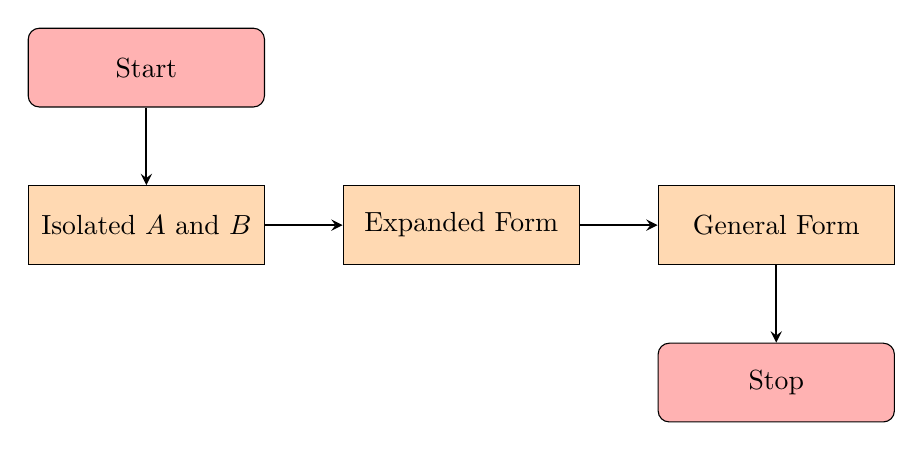
\begin{tikzpicture}[node distance=2cm]
  \node (start) [startstop] {Start};
  \node (pro1)  [process, below of=start] {Isolated $A$ and $B$};
  \node (pro2)  [process, right of=pro1, xshift=2cm] {Expanded Form};
  \node (pro3)  [process, right of=pro2, xshift=2cm] {General Form};
  \node (stop)  [startstop, below of=pro3] {Stop};

  \draw [arrow] (start) -- (pro1);
  \draw [arrow] (pro1) -- (pro2);
  \draw [arrow] (pro2) -- (pro3);
  \draw [arrow] (pro3) -- (stop);
\end{tikzpicture}
\caption{Metamorphosis of Value forms.}
\label{fc:metamorform}
\end{fccontainer}

The antipodal form of Value, relative and equivalent forms, seems to acquire this antagonistic nature since its inception in the Elementary form of Value.  The fact that the equation \ref{eq:exchangemean} can be read forwards and backwards, and as remarked in \ref{rem:valexchvalform}, the antipodal contrast is difficult to grasp.

The Expanded form of Value, where reversibility of the equation is contrained, polar contrast is clear.  A single commodity can now completely expand its relative value and it acquires expanded form by the virtue of all other commodites playing the role of equivalents.  Once the reversibility is restored, Karl exclaims, Expended form converts into General form of Value.

Finally, the General form of Value gives the world of commodities a ``general social relative form'' of Value.  Here one commodity becomes Universal Equivalent and others are equivalent, meaning, only the Universal Equivalent commodity (say $A$) has the ability to be directly exchangeable with rest of the commodities.  The commodity $A$ is no longer in the relative value form.  Karl reasons that if $A$ were to be endowed with relative form, whilst being Universal Equivalent, it would imply that $A$ serves as its own equivalent (I don't know how).  A contradiction in Marxist thought!  Karl sees no fun in this tautology because there is no capture of Value and its magnitude.

We, on the merry hand, have no issue with this.  In fact this patches up couple of holes we encountered while branching off from Marxist thought.  They are as follows
\begin{itemize}
\item My disagreement, in remark \ref{mark:reflexarg}, propogating the reflexive agenda.
\item My definition of generalization written in \ref{sec:newgenvalform}.
\end{itemize}

Karl states that in order to express the relative value (see \ref{def:relval}) of Universal Equivalent we must reverse the General form equation \ref{eq:genformval}, like so in my imagination
\begin{equation}
  \left(
  (\text{np})_{\text{coat}} = \begin{cases*} 
    2\cdot (10\text{yd})_{\text{linen}}\\
     (10\text{lbs})_{\text{tea}}\\
      \ldots
   \end{cases*}\right)^\omega.
\end{equation}
Still this Universal equivalent has no ``relative form of Value'' common with other commodities, thus
\begin{equation}
  \left(
  \underbrace{(\text{np})_{\text{coat}}}_{\text{\st{relative form}}} = \begin{cases*} 
    2\cdot (10\text{yd})_{\text{linen}}\\
     (10\text{lbs})_{\text{tea}}\\
      \ldots
   \end{cases*}\right)^\omega.
\end{equation}
 Karl's claim is that the relative value (Value is relatively expressed [sic]) is in the never ending series of other commodities.  This is precisely the Expanded form of relative value ``showing itself as the specific from of relative value for (Universal) equivalent commodity''.

I will visit this topic after coming back with full mathematical formulation and check how philosophy and logic go together and does my own version do any reconciliation.

\bibliographystyle{JHEP.bst}
\bibliography{list.bib}

\appendix

\section{Word Meanings}
company $\rightarrow$ con pane (Italian) $\rightarrow$ Group of people eating bread and doing business.\newline
finance $\rightarrow$ finir (French) $\rightarrow$ paying off blood debts and finishing the tangible commercial transactions, means to achieve the end of an activity or something.

\end{document}